\section{Introduction}
The Internet is a land of mistrust for good reasons, yet it's often required to trust each other. 

A common example for the use of commitment-schemes is the \textit{coin-toss via telephone}: Alice declares her call, and Bob tosses the coin. However, Alice is unable to \textit{see} the real coin-toss and relies on Bobs righteousness - which is a pretty bad idea. 

Evil Bobs can simply declare the wrong toss for Alice' call, making her loose every single time. Overall Bob can manipulate the outcome easily by choice with his knowledge of Alice' call. 

Therefore Alice needs to hide her prediction. A simple way of \textit{saving} Alice from manipulation is that Alice declares her call \textit{after} Bob announces the coin-toss-outcome. Needless to say, now Alice is in the position to make her calls in her favor every time, which is not acceptable for Bob. 

~\newline Commitment-schemes enable both parties to a \textit{fair-play} and tools to detect manipulation creating relative trust. In a successful commitment, Alice hides her guess with kryptographic measures and sends it to Bob. Bob then declares the coin-toss to Alice, without knowledge of her call. At this point Alice knows, if she has won or lost, and enables Bob to read her guess by sending the required keys for decryption.

At this point both parties know the \textit{real} outcome and the real winner of the coin toss. The measures if any manipulation is detected are beyond this protocol.

~\newline There are several cases where commitment-schemes are commonly used, for example in \textit{challenge and response}-authentication, whereof a simple example is provided at the end of this paper in section \ref{sec:casestudy}.

Also, other higher protocols require commitments, such as \textit{secret-sharing}. Unfortunately these protocols are out of scope for this paper. 

\subsection{Protocol}
The following steps are considered the basic protocol of commitment-schemes and vary only in their implementation. Often the protocol is shortened to only two steps, the commitment and the reveal (step 1 and 3), as these are the only steps requiring communication. This shortened version is also depicted in figure \ref{fig:protocoll}.  
\begin{enumerate}
	\item A \textbf{commits} to B
	\item B keeps commitment, unable to read or process it
	\item A \textbf{reveals} to B
	\item B verifies the commitment 
\end{enumerate}
To elaborate this protocol, we use another common picture as shown in figure \ref{fig:protocoll}: putting a message in an unbreakable, non-transparent and locked box (shown in the \textit{setup-step} of the figure).

For \textit{step 1} of the protocol, Alice \textbf{commits} the box to Bob. Bob cannot see or alter the message inside the box. Picking up the example of the \textit{coin-toss via telephone}, after \textit{step 2} Bob would announce the outcome to Alice.
 
For \textit{step 3} of the protocol, Alice \textbf{reveals} the commitment to Bob, sending him the key for the box (and commonly sending the message as well, proving that she is not only in possession of the key but also the secret itself). 

If the key \textit{fits}, Bob is able to unlock the box in \textit{step 4} and compare the message provided by Alice with the message found in the box. 
\begin{figure}
	\centering
	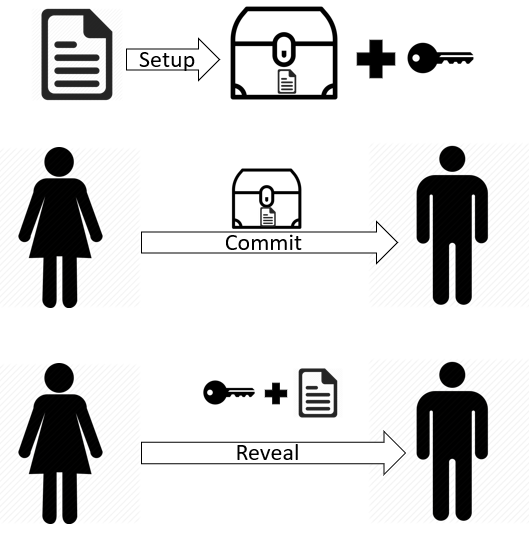
\includegraphics[width=0.8\linewidth]{Images/protocoll}
	\caption[Commitments]{Commitments}
	\label{fig:protocoll}
\end{figure}

\subsection{Attributes}
The following attributes are required for commitment-schemes to be secure and successfully fulfill their purpose:

\begin{enumerate}
	\item \textbf{Binding:} The values Alice put in the commitment cannot be changed after Bob recieved it 
	\item \textbf{Hiding:} Bob cannot gain any information about the message from the commitment itself
	\item \textbf{Viability:} If both parties follow the protocol correct, Bob is always able to recover the committed value
\end{enumerate}
Except for viability, the fulfillment of each attribute will be shortly discussed in the regarding implementations. 

~\newline For elaboration, the image of the box is fitting aswell: 

Once locked inside the box, the message cannot be altered by Alice (or any other party). After she commits it, Alice is \textbf{bound} to the value, as there can never be a different value inside the box after this point. 

Through the attributes \textit{non-transparent and unbreakable} of the box, the \textbf{hiding}-attribute of the protocol is fulfilled: Bob cannot look into the box and does not know anything about the message if he does not have the key. The only way to properly gain knowledge about the message is the key provided by Alice. 

The \textbf{viability} is given, as \textbf{only} the (correct) key will open the box. The correct key will always open the regarding boy, and no other key will \textit{ever} be able to unlock the message. 

~\newline There are two additional attributes based on the fact that we are working with computers:
\begin{enumerate}
	\item Bobs are able compare commitments.
	\item Commitments are \textit{tradeable} and replicable - both for Alice and Bob, still keeping their primary attributes and are fully functional. This attribute is vital for the case study presented in section \ref{sec:casestudy}.
\end{enumerate}

~\newline The trading can be displayed with the box: If $Bob_1$ decides to give the box to $Bob_2$, $Bob_2$ is also unable to read or open it. Alice can now also contact $Bob_2$ with the key and the message, to which $Bob_2$ can open the box and compare the message, just like $Bob_1$ would do. 

Also Alice is able to trade her key and message to any $Alice_2$, which enables $Alice_2$ to reveal her like the $real$ Alice would. 

~\newline The ability to copy and compare commitments is not applicable to the example of the locked box. However, as most commitments rely on numbers, the \textit{real} commitment consists of bits and therefore are easily duplicated. 

For the comparison it's to add, that it's possible to have the same commitment for a different combination of messages and keys. However, as the key's should be chosen randomly, these collisions are highly unlikely (in case of the hash-based implementations as likely as hash-collisions themselves). 
\subsection{Additional Security-Measures}
There are several \textit{best-practices} which are not functional for the protocol itself, but are necessary to secure any party involved in the protocol and any application using the protocols. They will be shortly summarized and explained: ~\newline

	\paragraph{commitments should be one- (positive-) use only} This originates from the \textit{reveal}-step, in which everything required to reveal the commitment successfully is transmitted. An eavesdropper would after the initial reveal be able to copy the required \textit{credentials} and also reveal the commitment correct.  To fix this issue, simply mark used commitments as deprecated (if they are further required), or delete them completely. 
	\paragraph{commitments should have a lifetime} (in time and/or tries)
	This behavior helps against brute-force attacks from exterior, given that the attacking party does not hold the commitment itself. If an aggressor has the commitment, he can start brute-force attacks locally (this holds true for eve and bob) which still requires \textbf{safe} cryptographic implementations.
	Additionally the lifetime (in e.g. days) is useful for Bob, as he has limited resources and should only keep \textit{required} information. 
	\paragraph{traded commitments to a third party should be deprecated directly with first reveal} This is an extended version of the problem shown in paragraph \textit{a)} of this subsection. Given there are multiple copies of the same commitment, and an eavesdropper knows the parties which hold a copy, Eve can successfully reveal the commitment to any party. For addressing this issue, the commitments need to be recursively deprecated throughout any party which the commitment was shared to. A common way to do this for Bob is to reveal the commitment by himself - this method does not require additional structures and also verifies that Bob knows the correct values. 
	
	However, if there is a larger number of parties involved, Eve can be \textit{faster} reaching to the last Bob and reveal the commitment. Additionally there are many attacks that disturb the communication between Bob's, thus leaving more chances for Eve to reveal herself as Alice. Sharing commitments should be therefore only used when required. 
	\paragraph{messages must contain random parts} This rather trivial point is important for any implementation to fulfill any attribute connected to the \textit{computational safeness} of hashfunctions and the discrete logarithm.  
~\newline ~\newline
For every implementation based on commitment-schemes all of the above should be taken to account. There are several problems if only a single point is left out, including identity theft and server-malfunctions. 

There are common libraries which support you in the goal of a secure implementation, e.g. an implementation in Haskell \cite{b0} . The use of an open-source and \textbf{maintained} library is highly recommended.